\documentclass[10pt]{beamer}

% Theme choice:
\usetheme{metropolis}
\definecolor{myblue}{RGB}{0, 100, 250} % Light blue color
\setbeamercolor{title}{fg=myblue}
\setbeamercolor{frametitle}{bg=myblue, fg=white}
\setbeamercolor{structure}{fg=myblue}
\usepackage[english]{babel}


% Title information
\title[3D Vision in Collaborative Robotics]{Application of 3D Vision in Collaborative Robotics for Automated Machine Feeding}
\author{Pedro Afonso \& Simão Ribeiro}
\date{\today}
\institute{Universidade de Aveiro \\ In Collaboration with Azevedos Indústria SA}

\begin{document}
	
	% Title slide
	\frame{\titlepage}
	
	% Introduction section
	\section{Introduction}
	\begin{frame}{Project Overview}
		\textbf{Background:}
		\begin{itemize}
			\item Cork trace orientation and automation are critical for improving cork production quality.
			\item Collaborative robotics integrated with 3D vision systems can revolutionize industrial automation.
		\end{itemize}
		\textbf{Project Objectives:}
		\begin{itemize}
			\item Develop a 3D vision system for mapping and identifying bulk cork pieces.
			\item Integrate the vision system with a collaborative robot for feeding production machines.
			\item Validate system performance in precision, efficiency, and safety.
		\end{itemize}
	\end{frame}
	
	% Problem analysis
	\section{Problem Analysis}
	\begin{frame}{Problem Analysis}
		\textbf{Challenges in Cork Industry:}
		\begin{itemize}
			\item Handling variability in size, shape, and orientation of cork pieces.
			\item Addressing natural variations in color, texture, and appearance due to cork being a natural product.
		\end{itemize}
		\textbf{User and Context:}
		\begin{itemize}
			\item Users: Manufacturers of cork stoppers.
			\item Context: Factory automation for cork production and finishing processes.
		\end{itemize}
		\textbf{Key Questions:}
		\begin{itemize}
			\item How can 3D vision systems enhance collaborative robot functionality?
			\item What methods ensure high precision in cork trace orientation detection?
		\end{itemize}
	\end{frame}
	
	% Computer Vision Techniques
	\section{Vision System Design}
	\begin{frame}{Computer Vision Techniques}
		\textbf{Techniques and Tools:}
		\begin{itemize}
			\item Point Cloud Processing: Filtering, segmentation, and clustering using \texttt{open3d}.
			\item Noise Removal: Statistical outlier removal for cleaner data.
			\item Clustering: Conditional Euclidean Clustering (CEC) to segment cork traces.
			\item RGB Mapping: Overlaying clusters onto RGB images for enhanced visualization.
		\end{itemize}
		\textbf{Justification:}
		\begin{itemize}
			\item Combines efficiency of traditional analytical methods with robustness of modern clustering.
			\item Suitable for handling variability in cork pieces.
		\end{itemize}
	\end{frame}
	
	% Implementation details
\section{Implementation}
\begin{frame}{System Workflow}
	\textbf{Workflow Stages:}
	\begin{enumerate}
		\item \textbf{Data Acquisition}: 3D point cloud capture using Intel RealSense D435i.
		\item \textbf{Pass-Through Filtering}: Reduce point cloud size by isolating regions of interest.
		\item \textbf{Floor Removal}: Segment and exclude planar surfaces to isolate cork pieces.
		\item \textbf{Downsampling}: Apply voxel grid filtering to reduce point cloud density.
		\item \textbf{Outlier Removal}: Eliminate noise using statistical outlier removal.
		\item \textbf{Clustering}: Use Conditional Euclidean Clustering (CEC) to detect cork piece groups.
		\item \textbf{Mapping}: Overlay clustered points onto RGB images for validation.
	\end{enumerate}
	%\includegraphics[width=\textwidth]{workflow_diagram.png} % Replace with actual diagram
\end{frame}
	
	\begin{frame}{Original Image}
		\textbf{Description:}
		\begin{itemize}
			\item Shows the unprocessed point cloud of the cork pieces.
			\item Captured using Intel RealSense D435i.
		\end{itemize}
		\begin{center}
			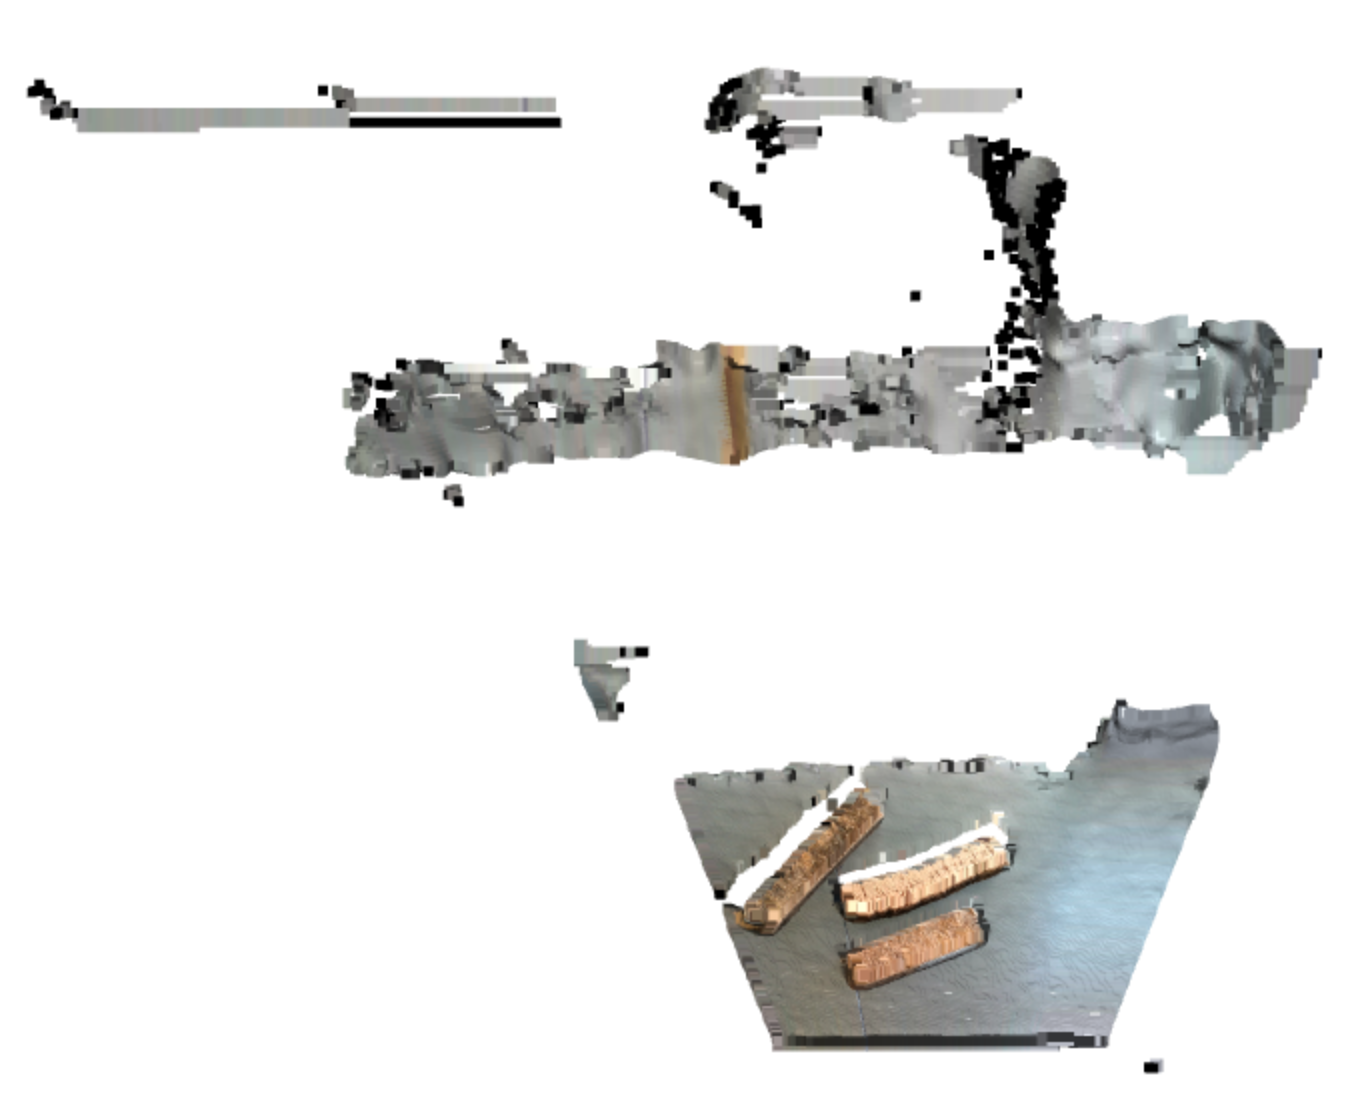
\includegraphics[width=0.5\textwidth]{img/original.png}
		\end{center}
		\textbf{Results:}
		\begin{itemize}
			\item Raw data ready for processing (no filtering or clustering applied yet).
		\end{itemize}
	\end{frame}
	
	% Slide 1: Pass-Through Filtering
	\begin{frame}{Pass-Through Filtering}
		\textbf{Description:}
		\begin{itemize}
			\item Reduces the dataset size by focusing on regions of interest.
			\item Filters applied along X, Y, and Z axes to isolate relevant points.
		\end{itemize}
		\begin{center}
			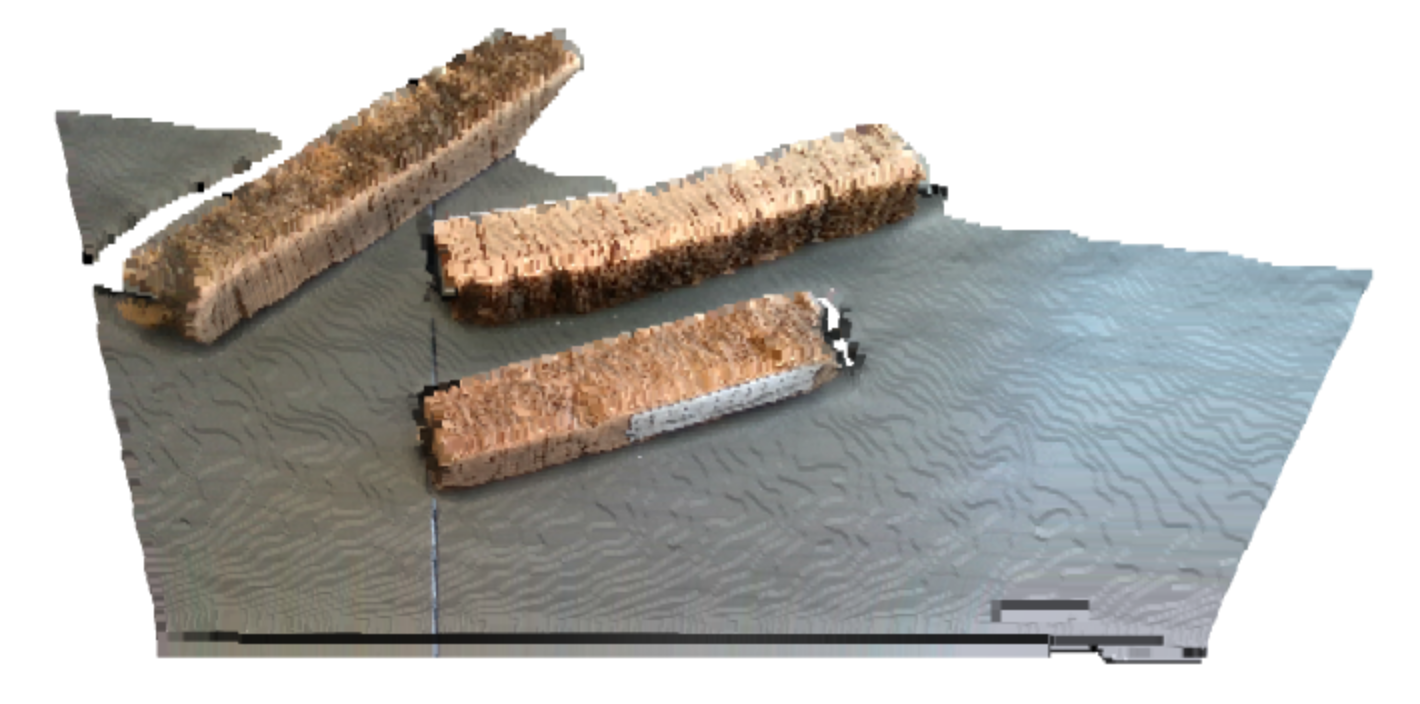
\includegraphics[width=0.7\textwidth]{img/passabanda.png}
		\end{center}
		\textbf{Results:}
		\begin{itemize}
			
			\item Significant reduction in point cloud size.
			\item Retained only the cork-relevant sections of the cloud.
		\end{itemize}
		\end{frame}
	
	% Slide 2: Floor Removal
	\begin{frame}{Floor Removal}
		\textbf{Description:}
		\begin{itemize}
			\item Identifies planar surfaces and removes them to isolate cork pieces.
			\item Utilizes RANSAC-based plane segmentation.
		\end{itemize}
			\begin{center} % Centers only the image
				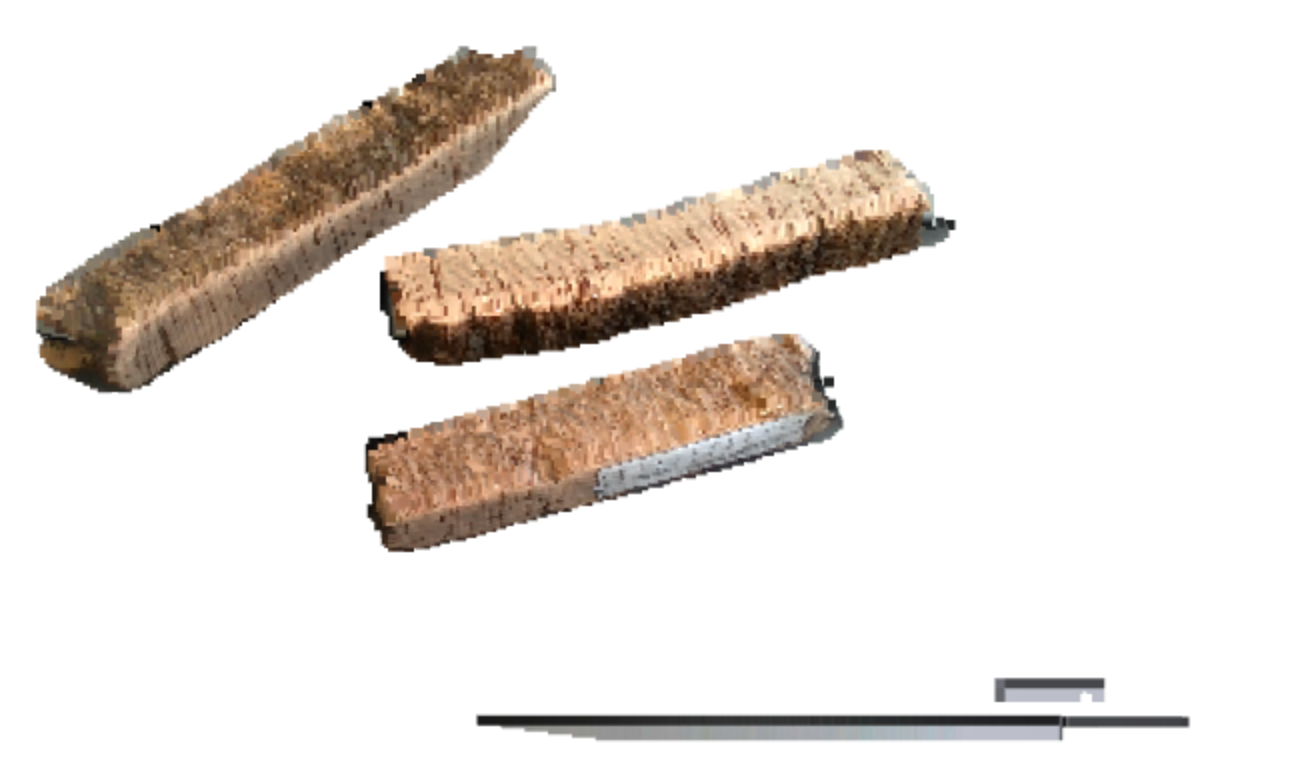
\includegraphics[width=0.6\textwidth]{img/background.png}
			\end{center}
			
		\textbf{Results:}
		\begin{itemize}
			\item Successfully excluded floor points.
			\item Enhanced focus on cork clusters in 3D space.
		\end{itemize}
		
	\end{frame}
	
% Slide 3: Downsampling and Noise Removal
\begin{frame}{Downsampling and Noise Removal}
	\textbf{Description:}
	\begin{itemize}
		\item Downsampling: Voxel grid reduces point cloud density for computational efficiency.
		\item Noise Removal: Statistical outlier removal eliminates scattered points.
	\end{itemize}
	
	%
	
	\begin{minipage}{0.42\textwidth} % First image occupies 48% of text width
		\centering
		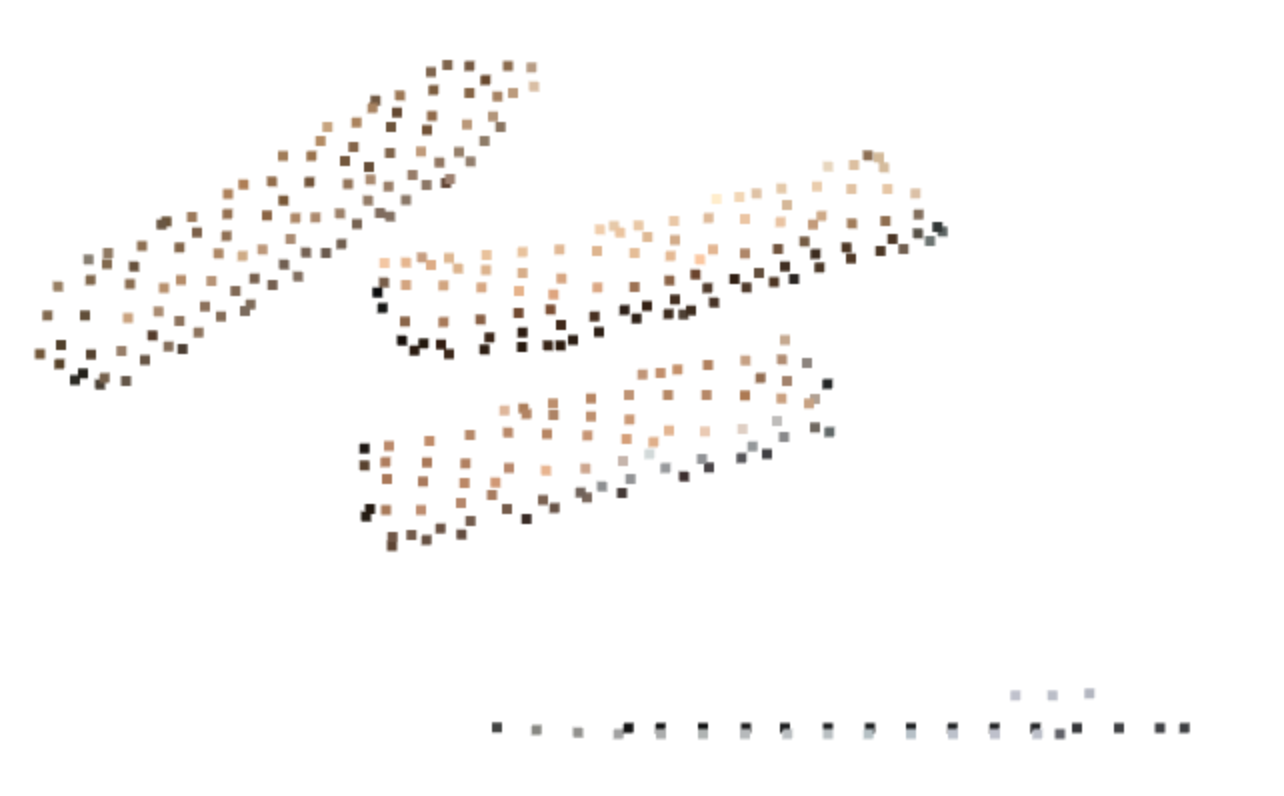
\includegraphics[width=\textwidth]{img/voxelGrid.png} % First image
		
	\end{minipage}
	\hfill % Adds horizontal space between images
	\begin{minipage}{0.42\textwidth} % Second image occupies 48% of text width
		\centering
		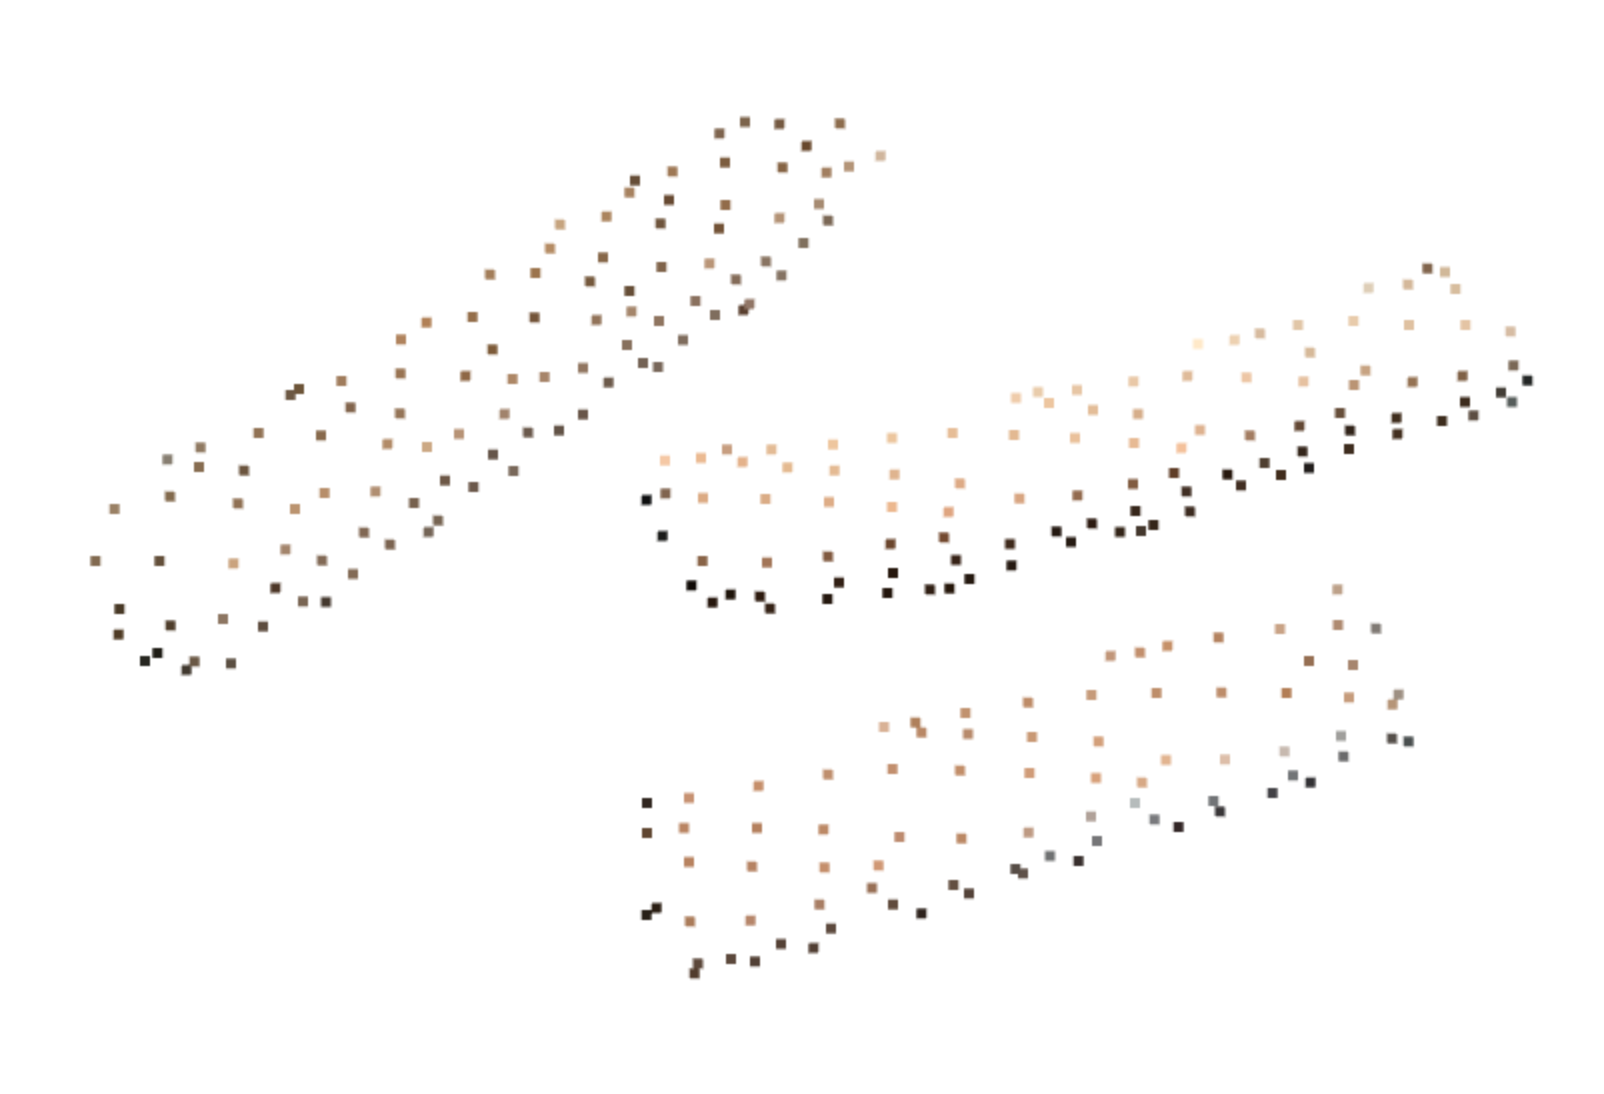
\includegraphics[width=\textwidth]{img/outlier.png} % Second image
	\end{minipage}
	
	\textbf{Results:}
	\begin{itemize}
		\item Downsampled point cloud retains key structural features.
		\item Improved clarity and accuracy for clustering stages.
	\end{itemize}
\end{frame}

	
% Slide 4: Clustering and Oriented Bounding Boxes
\begin{frame}{Clustering and Oriented Bounding Boxes}
	\textbf{Description:}
	\begin{itemize}
		\item \textbf{Clustering:} Applied Conditional Euclidean Clustering (CEC) to segment cork pieces.
		\item \textbf{OBBs:} Generated Oriented Bounding Boxes to define spatial extent and orientation of clusters.
	\end{itemize}
	\begin{center}
		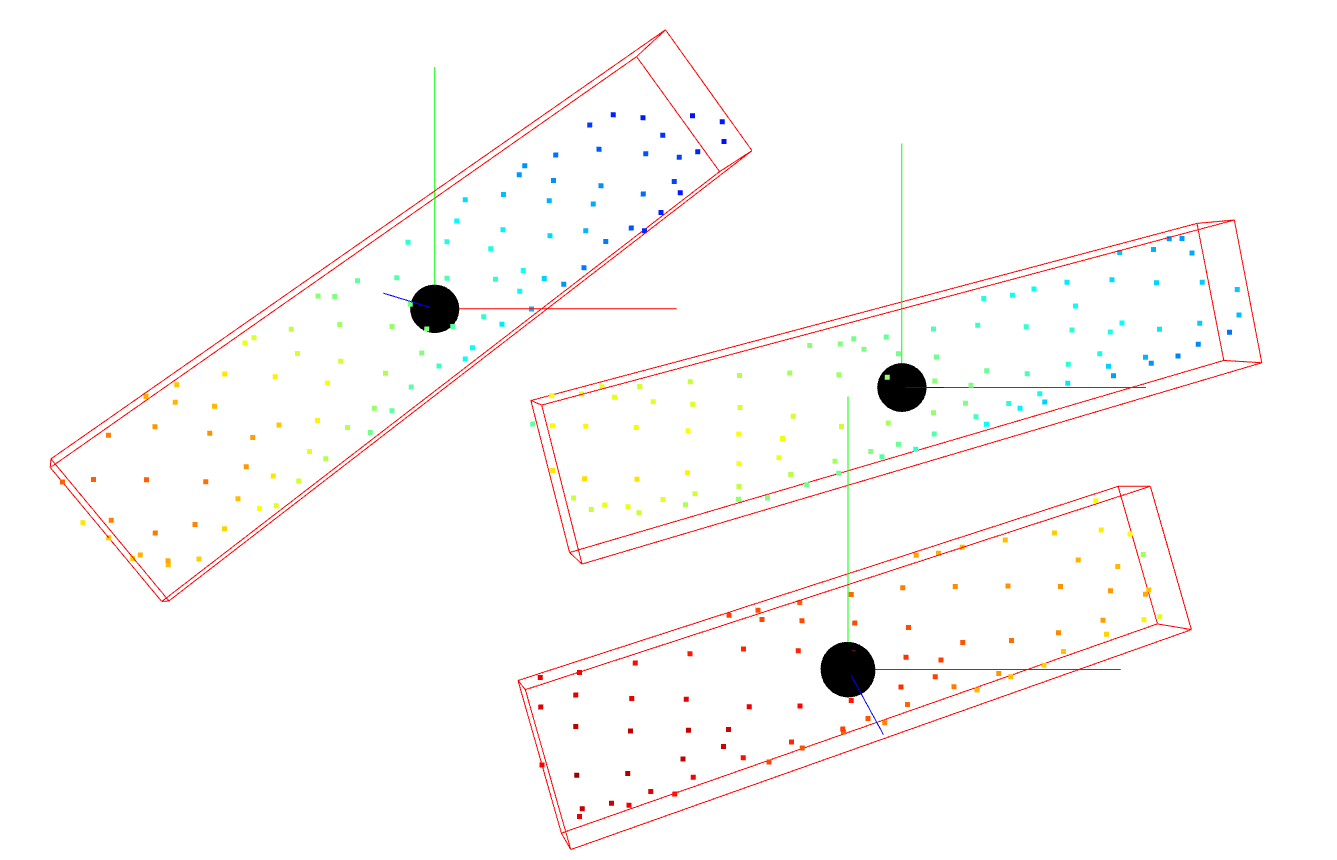
\includegraphics[width=0.4\textwidth]{img/bb.png} % Adjusted image size
	\end{center}
	
	\textbf{Results:}
	\begin{itemize}
		\item Segmented cork pieces into clusters using CEC.
		\item OBBs accurately defined cluster orientations.
		\item Ready for further analysis, such as face detection.
	\end{itemize}
\end{frame}


	
	% Slide 5: RGB Masking
	\begin{frame}{Mapping and Masking onto RGB Image}
		\textbf{Description:}
		\begin{itemize}
			\item Projected 3D clusters onto the 2D image plane.
			\item Created a smooth green mask overlaid onto the RGB image.
		\end{itemize}
		\begin{minipage}{0.48\textwidth} % First image occupies 48% of text width
			\centering
			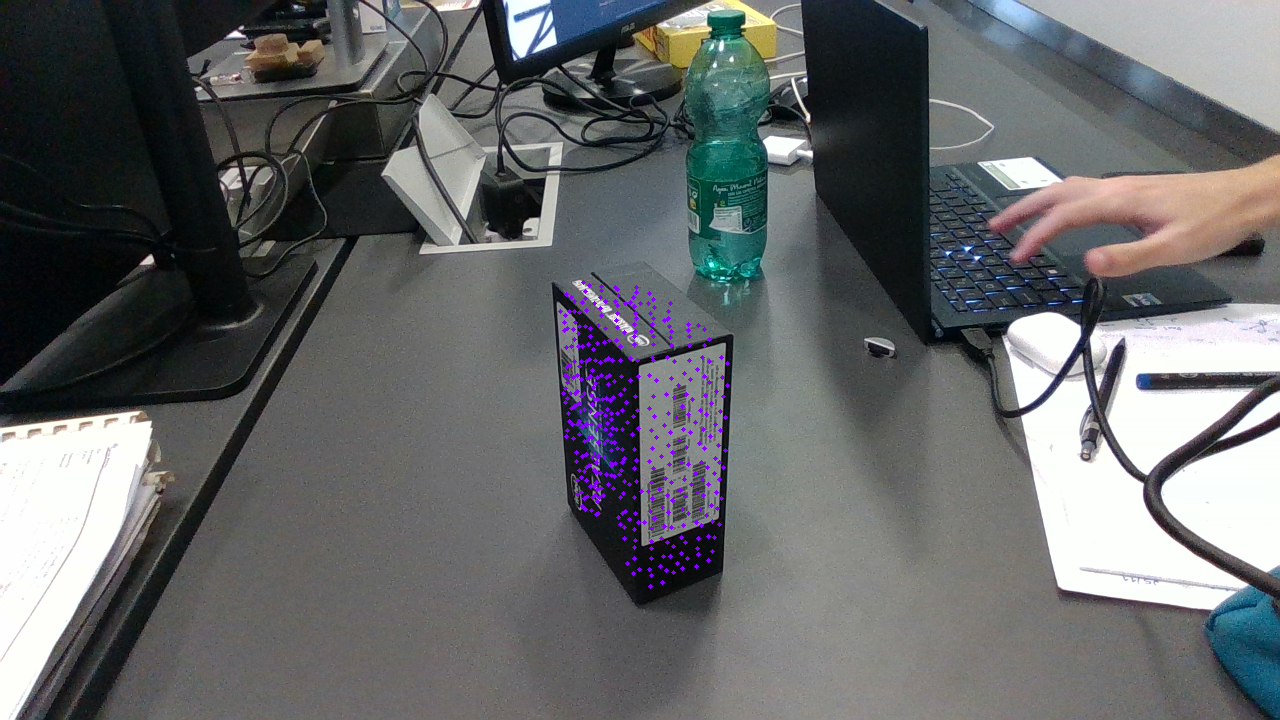
\includegraphics[width=\textwidth]{img/points.png} % First image
			
		\end{minipage}
		\hfill % Adds horizontal space between images
		\begin{minipage}{0.48\textwidth} % Second image occupies 48% of text width
			\centering
			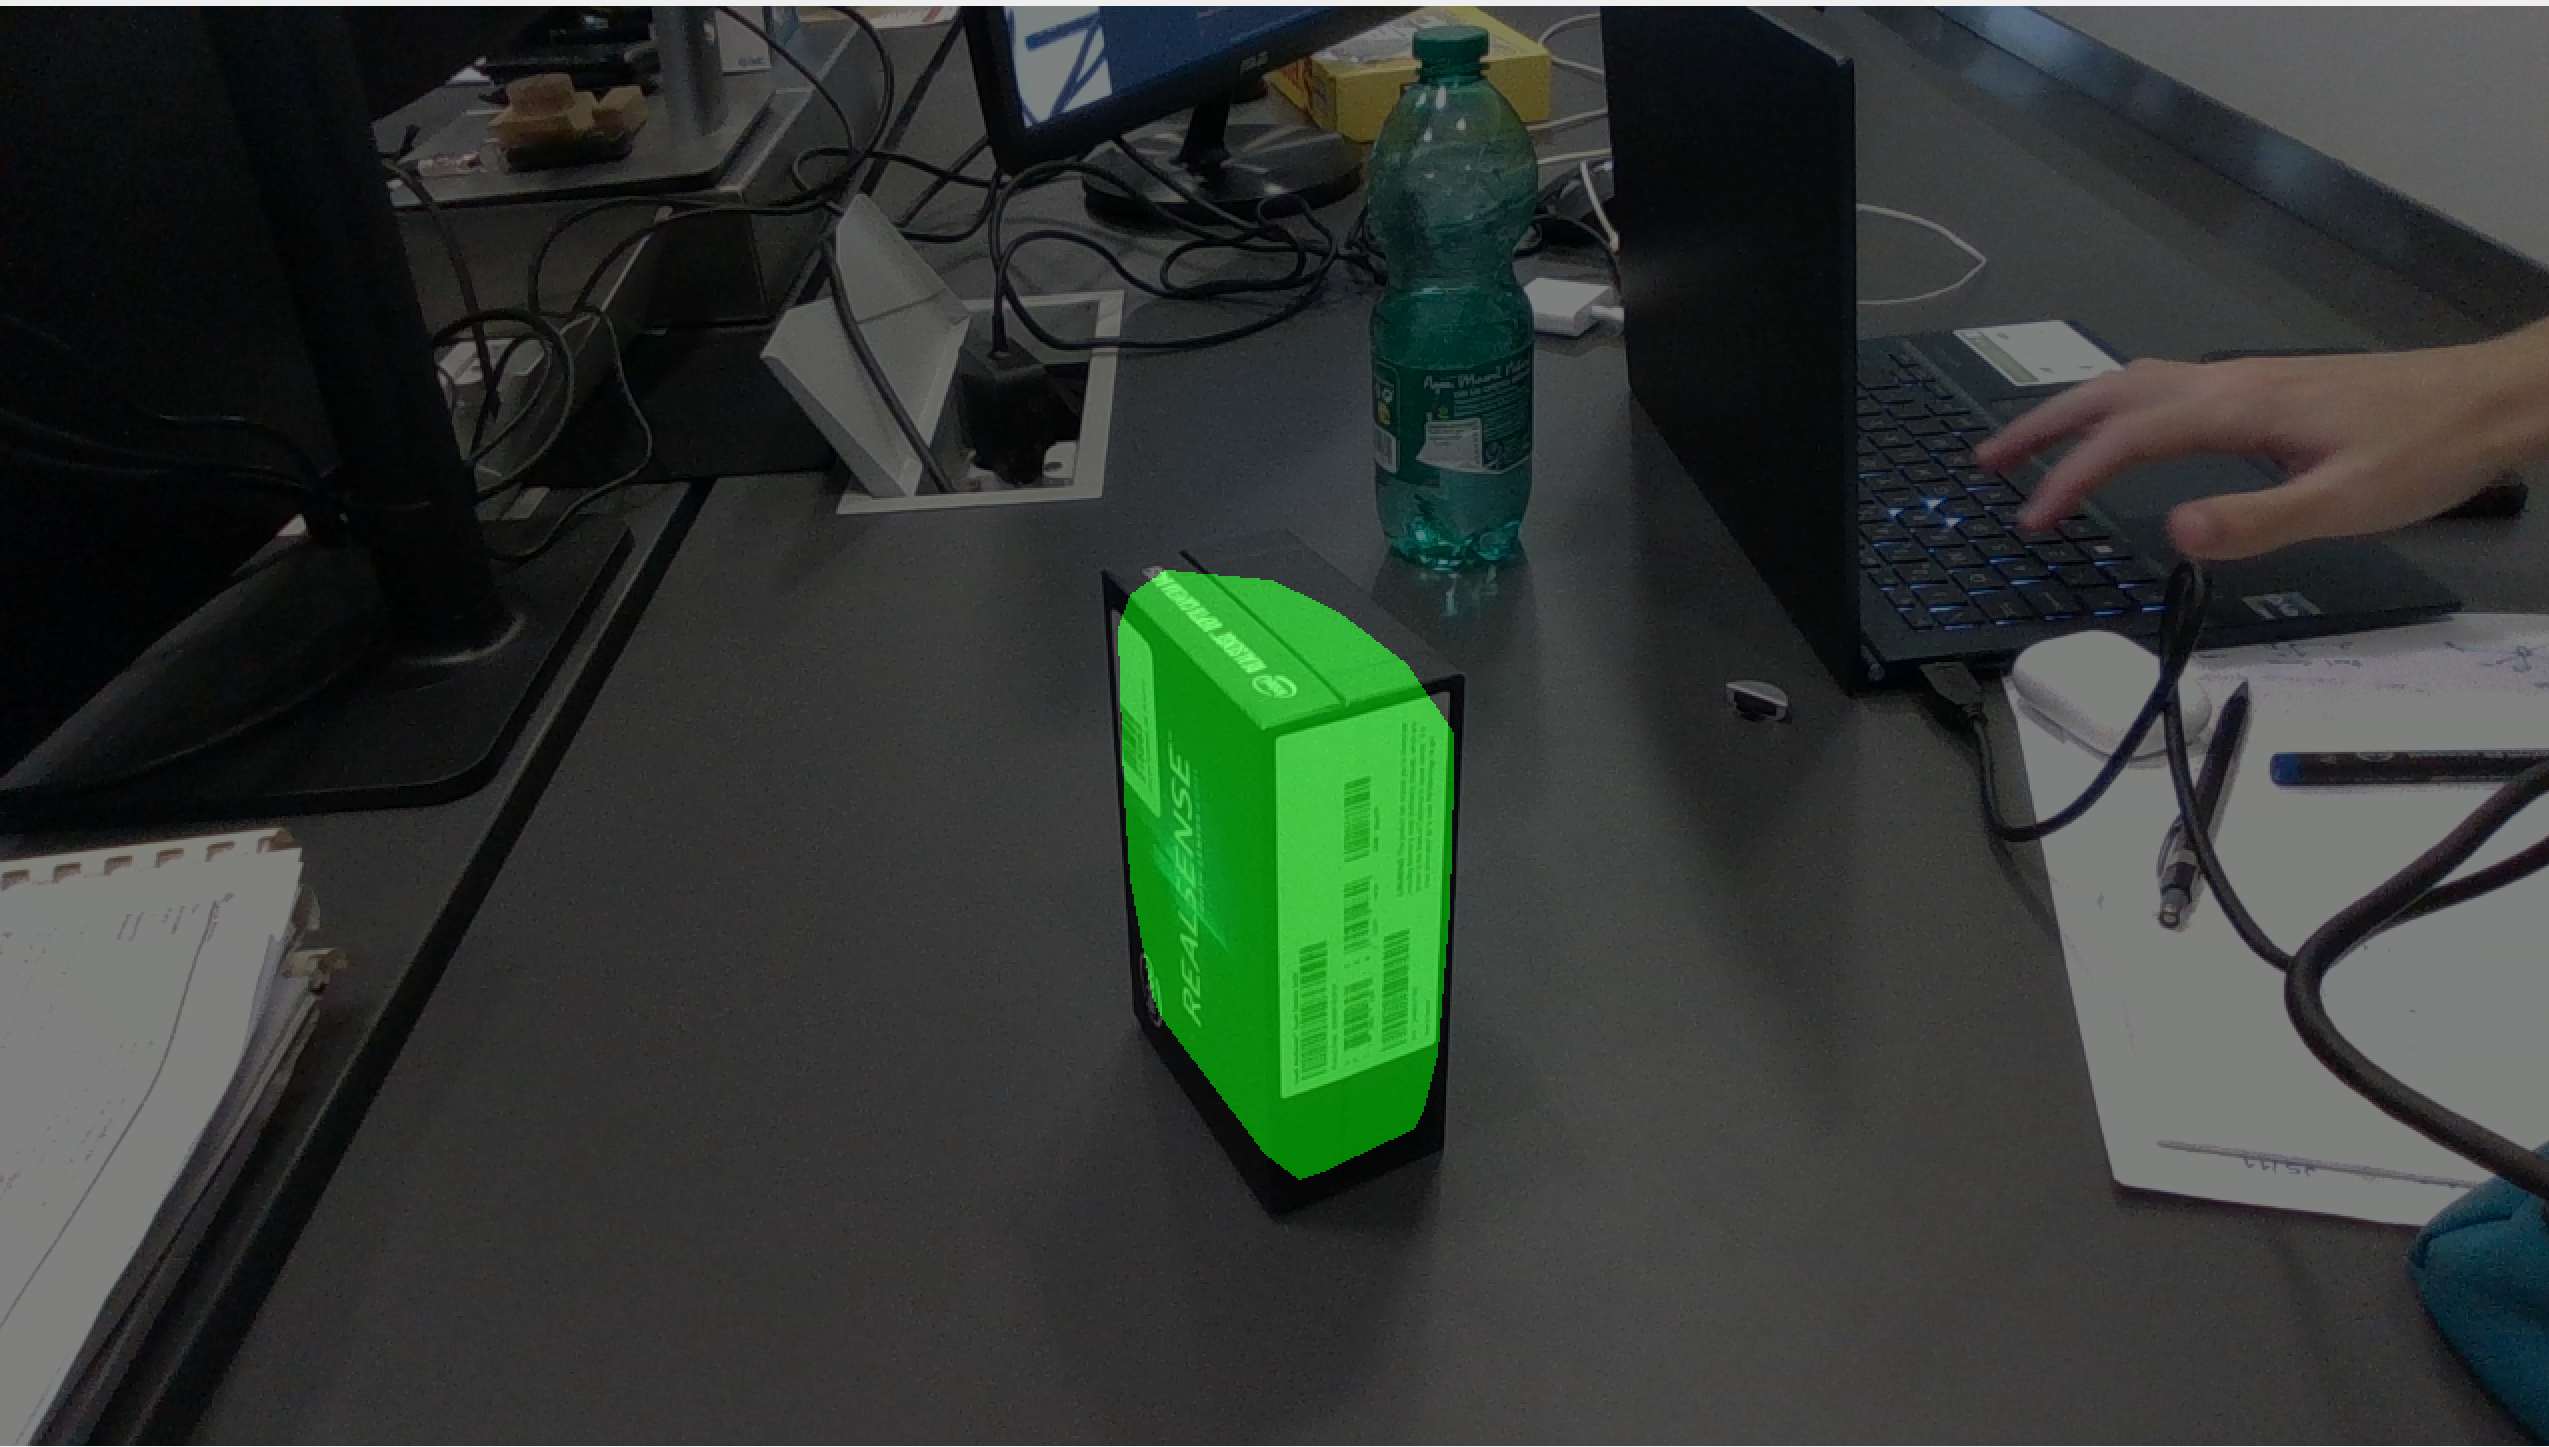
\includegraphics[width=\textwidth]{img/mask.png} % Second image
		\end{minipage}
	
		\vspace{0.5cm} % Adds vertical space between description and images
		
		\textbf{Results:}
		\begin{itemize}
			\item Enhanced visualization of cork cluster regions.
			\item Provided a foundation for future Machine Learning integration.
		\end{itemize}
		%\includegraphics[width=\textwidth]{rgb_masking_results.png} % Replace with your actual figure
	\end{frame}

	\section{Results and Analysis}
	\begin{frame}{Preliminary Results Overview}
		\textbf{Successes:}
		\begin{itemize}
			\item Segmentation and clustering of cork pieces using 3D vision techniques.
			\item Effective overlay of processed clusters onto the RGB image.
		\end{itemize}
		\textbf{Future Challenges:}
		\begin{itemize}
			\item Improve the quality of the images (Hole filling, Post Processing Filters, Laser projector settings).
			\item Identify and segment individual faces of the cork strips (e.g., top, sides).
			\item Extract the largest rectangle from the identified faces to enable feature extraction.
			\item Develop robust feature extraction for machine learning models to detect the back of cork strips.
		\end{itemize}
	\end{frame}
	
\section{Conclusion and Future Work}
\begin{frame}{Conclusion}
	\begin{itemize}
		\item Developed a pipeline up to the RGB masking stage for cork piece segmentation and visualization.
		\item Demonstrated effective clustering and initial masking techniques.
		%\item Identified limitations in clustering accuracy and segmentation of complete cork pieces.
		\item Set the foundation for extracting features required for machine learning-based orientation detection.
	\end{itemize}
\end{frame}

\begin{frame}{Future Work}
	\textbf{Immediate Goals:}
	\begin{itemize}
		\item Enhance image acquisition techniques to ensure cork pieces are captured with more detail.
		\item Implement segmentation techniques to identify individual faces (top, side, etc.) of the cork pieces.
		\item Extract geometric features from identified faces to prepare for machine learning models.
	\end{itemize}
	\textbf{Long-Term Goals:}
	\begin{itemize}
		\item Optimize the pipeline for real-time processing.
		\item Develop and train machine learning models for cork orientation detection using extracted features.
		%\item Expand the system to handle broader variations in cork geometries and other material types.
	\end{itemize}
\end{frame}

	
\end{document}
